%% arVM paper draft
\documentclass[letterpaper,twocolumn,10pt]{article}
\usepackage{usenix}
\usepackage{amsmath,amssymb,graphicx}
\hypersetup{hidelinks,pdftitle={arVM: Compiling Agent Plans for CXL Memory Sharing},pdfauthor={}}
\pagestyle{plain}
\frenchspacing
\AtBeginDocument{\typeout{ARVM-FORMAT: textwidth=\the\textwidth; textheight=\the\textheight; columnsep=\the\columnsep; baseline=\the\baselineskip; font=\csname f@size\endcsname pt}}

\AtBeginDocument{%
  \providecommand\BibTeX{{%
    Bib\TeX}}}

\usepackage{booktabs}
\usepackage{array}
\usepackage{tikz}
\usepackage{xspace}
\usetikzlibrary{positioning,fit,arrows.meta,calc}

\newcommand{\arvm}{arVM\xspace}
\newcommand{\cxl}{CXL\xspace}
\newcommand{\rag}{RAG\xspace}
\newcommand{\mlir}{MLIR\xspace}
\newcommand{\circt}{CIRCT\xspace}
\newcommand{\muse}{MUSE\xspace}
\newcommand{\dsec}{DSec\xspace}
\newcommand{\memtrade}{MemTrade\xspace}
\emergencystretch=2em
\vfuzz=2pt
% Generated from validated profile summary; do not edit numeric claims by hand.
\newcommand{\ProfileEpisodes}{12}
\newcommand{\ProfileSessions}{84}
\newcommand{\ProfileEvents}{484}
\newcommand{\ProfileProtocol}{11}
\newcommand{\ProfileIdleOneReads}{62}
\newcommand{\ProfileIdleOneDenominator}{103}
\newcommand{\ProfileIdleOnePercent}{60.2}
\newcommand{\ProfileCorpusKiB}{43.6}
\newcommand{\ProfileTwoScopeKiB}{575.7}
\newcommand{\ProfileTwoGraphKiB}{446.5}
\newcommand{\ProfileTwoSaving}{22.4}
\newcommand{\ProfileTwoReplaySaving}{22.2}
\newcommand{\ProfileTwoSharedPercent}{75.7}
\newcommand{\ProfileTwoSpanSeconds}{19.7}
\newcommand{\ProfileTwoActiveMillis}{24.2}
\newcommand{\ProfileFourScopeKiB}{959.6}
\newcommand{\ProfileFourGraphKiB}{736.4}
\newcommand{\ProfileFourSaving}{23.3}
\newcommand{\ProfileFourReplaySaving}{23.3}
\newcommand{\ProfileFourSharedPercent}{77.3}
\newcommand{\ProfileFourSpanSeconds}{37.4}
\newcommand{\ProfileFourActiveMillis}{43.4}


\begin{document}

\title{\arvm: Compiling Agent Plans for CXL Memory Sharing}

\author{{\rm Anonymous submission}}
\date{}
\maketitle

\begin{abstract}
Agent workflows retain retrieved documents and tool outputs across branches
and model calls. Private copies duplicate payloads; activity measurements
alone do not identify shared versions or future readers. We present \arvm,
a compiler and runtime design
that turns accepted agent plans into memory contracts for a CXL pool.
A data-movement graph names object versions, readers, and access scopes.
The compiler derives sharing and lifetime constraints, reserves bounded
outputs, and supplies placement hints before the next phase starts.
The runtime revalidates each contract against current object state and
memory pressure. This separates required references from speculative reuse,
so replanning can discard hints without releasing live data.
We prototype graph validation and admission, and measure native CXL sharing
and phase replay separately. Across 30 data-stage conditions, the geometric mean speedup over
copying into reused DRAM buffers is $1.129\times$. An eight-worker case
removes 32\,MiB of private copies at near-parity latency. Phase replay shows
both the benefit of timely lookahead and the traffic cost of wrong hints.
We additionally run \ProfileEpisodes{} multi-round OpenCode episodes over
CXL shared state. Tracking accepted object uses reduces median managed
payload occupancy by \ProfileTwoSaving--\ProfileFourSaving\% relative to
scope-only retention. The experiments establish sharing and lifetime behavior,
not an end-to-end inference speedup.
\end{abstract}

\section{Introduction}

An agent's data often outlives the tool call that produced it. Retrieved
passages feed several analysis branches; a repository snapshot is revisited
after a test; branch results remain live until synthesis completes. Giving
each worker a private copy simplifies execution but duplicates memory and
transfer work. Keeping all copies in local DRAM also ties a session's memory
footprint to its retained state, even while the agent waits for its next action.

MUSE and DSec motivate this workload. MUSE Code combines tool execution with
workspace permissions and sandbox enforcement \cite{musepermissions}.
DSec manages stateful agent sandboxes, including sharing, reclamation, and
state retention across training interruptions \cite{dsec2026}. We consider
how such workloads could use a CXL pool. These systems motivate the execution
and isolation requirements; they are not evidence of a CXL implementation.

The immediate opportunity is object sharing. Two authorized branches that read the same passage
version can map one backing allocation. Yet sharing alone does not determine
where that allocation should reside, whether a local replica is worthwhile,
or when the runtime can release it. Those decisions depend on the consumers
and on uses that cross tool-call boundaries.

\textbf{An accepted plan provides a view of the next memory phase.}
Once an agent selects its next actions, the harness can resolve some of their
inputs and dependencies before dispatch. Agentic RAG then resembles a FaaS
workflow DAG: retrieval produces evidence, parallel tasks consume it, and
synthesis consumes their results. Workflow systems such as SONIC already use
dependencies to optimize data passing \cite{sonic2021}. For memory management,
the graph must additionally name shared object versions and distinguish
active readers, pending uses, and state retained for a later round.

The same plan offers a limited opportunity to move data before use. An input
known before dispatch can be staged during the available interval; a finished
branch can release temporary capacity. This complements the feedback-driven
approach in \memtrade, which harvests and matches idle memory using observed
application performance \cite{memtrade2021}. Activity measurements describe
current pressure. Object dependencies supply different information: which
consumers share backing and which accepted operations will need it next.

The difficulty is that plans are partial and change during execution.
A retrieval result can enlarge the next context; a failed tool can introduce
a retry. Predicted reuse cannot justify freeing live data, and a candidate
placement can become stale before admission. \arvm therefore compiles each
accepted fragment into a \emph{memory contract}: object versions, access
requirements, input pins, capacity bounds, and optional placement hints.
The runtime validates the contract when it admits work and uses current
pressure to decide which optional actions to accept. Replanning changes
unstarted work while preserving references held by running tasks.

This paper makes three contributions:
\begin{itemize}
  \item An object-based data-movement graph that separates task dependencies
  from physical backing and records the scope of sharing.
  \item A compiler--runtime contract that separates required memory from
  speculative placement, with version checks and atomic admission.
  \item Real CXL measurements of sharing, phase lookahead, and compilation,
  plus live-agent traces and a future-use retention ablation.
\end{itemize}

The measurements support a conditional result: sharing can remove duplicate
DRAM without sacrificing data-stage latency, and lookahead can hide movement
when the next input is known early enough. They do not establish a complete
agent speedup or an improvement over a deployed \memtrade controller.

\section{Motivation}

\subsection{State Lifetime Crosses Execution Phases}

A coding agent can revisit shared source after a model call or a peer's
analysis. MUSE's workspace scopes and DSec's retained sandboxes motivate
distinguishing authorization from state lifetime \cite{musepermissions,dsec2026}.
We measure this distinction with real OpenCode tool calls: two or four
reviewer roles inspect a common source snapshot, publish drafts, cross-read
a peer's draft, publish reviews, and hand them to a synthesizer. The task
fragment is prescribed; the model executes the calls and writes the findings.

With two and four reviewers, the shared source version spans a median
\ProfileTwoSpanSeconds{} and \ProfileFourSpanSeconds{} seconds between its
first and last reads, while access critical sections total only
\ProfileTwoActiveMillis{} and \ProfileFourActiveMillis{} milliseconds.
These are intervals in the instrumented data path, not CPU-idle or bus-traffic
measurements. An object can be untouched yet required by an accepted future
consumer. Conversely, scratch data can become dead while its owner continues
in a later review phase.

\subsection{A Partial DAG Is Enough to Expose Sharing}

Figure~\ref{fig:observed-profile} reconstructs object-version edges from one
measured episode. Common-source fanout, peer exchange, and final fan-in are
different relationships even when the tool names and access scopes match.
Under dataflow retention, \ProfileTwoSharedPercent\% and
\ProfileFourSharedPercent\% of nonempty reads consume versions read by
multiple logical agents. These are properties of the specified tasks, not
estimates of sharing prevalence in natural workloads.

As in workflow data passing \cite{sonic2021}, named producer--consumer edges
expose reuse. For memory management, the edges must also identify versions,
backing aliases, and remaining uses. A broad read permission is not a future
use; a lock protects a current operation but does not identify its last
consumer. Equivalent effect/reference tables can encode this information;
the experiment motivates the information, not a uniquely necessary graph
representation. Unknown future turns still require session roots or recovery
backing rather than speculative reclamation.

\begin{figure*}[t]
\centering
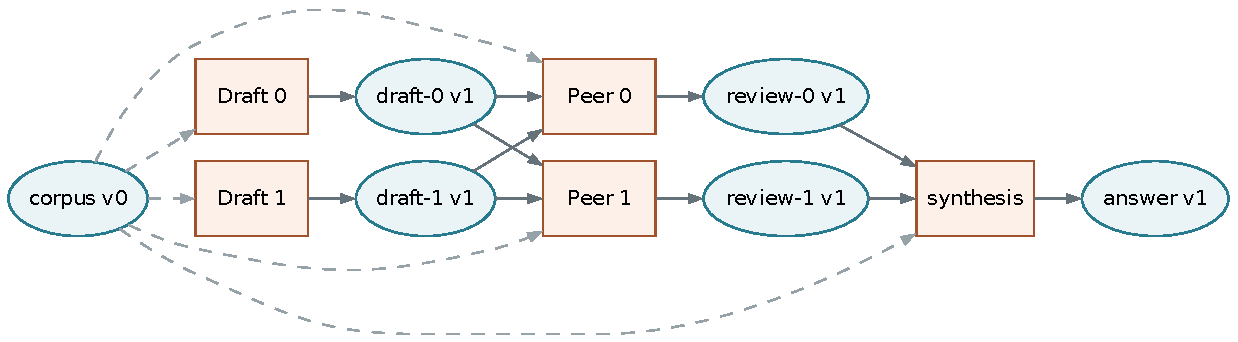
\includegraphics[width=\textwidth,height=2.05in,keepaspectratio]{figures/profile-observed-dataflow.pdf}
\caption{Observed CXL object-version dataflow in the median-duration
two-reviewer dataflow episode. Boxes are real OpenCode task sessions;
ellipses are shared versions. Dashed edges are common-source reads, and
solid edges are observed publications or reads of produced versions.
Private scratch, the mutable audit ledger, and empty CAS reads are omitted
only from this view. The complete trace includes them.}
\label{fig:observed-profile}
\end{figure*}

\subsection{Planning Exposes a Placement Opportunity}

Pooling assigns capacity among consumers; sharing lets authorized consumers
use common backing. CXL supports different combinations of these mechanisms
depending on the platform \cite{cxlsharing2023}. Our first target is one host
whose workers can map a common CXL region. It does not require cross-host
coherence or a new fabric protocol.

Between resolving an input and starting its consumer, the runtime may have
time to create mappings, stage data, or reserve local capacity. We call this
interval the \emph{planning lead time}. It begins when the relevant input
becomes known, not when an LLM starts reasoning. A long model call gives no
useful lookahead if its output is needed to identify the next input.

The opportunity is conditional. Repeated reads can favor a DRAM replica;
contending transfers can erase a prefetch benefit; a changed plan can waste
bandwidth. \arvm uses accepted dependencies to establish required references
and uses predicted timing only to rank optional actions. Section~\ref{sec:evaluation}
measures these effects separately so that a capacity saving is not mistaken
for a universal latency improvement.

\section{System Model and Architecture}
\label{sec:architecture}

\subsection{Scope and Assumptions}

The first target is a single host with local DRAM, an OS-visible CXL memory
region, and several isolated agent workers. A trusted runtime controls object
allocation and maps selected regions into workers. The memory controller can
adjust placements and local budgets without changing the agent's chosen tools
or model inputs. Accelerators remain separate consumers that may require
explicit staging. A CXL region is neither an unlimited heap nor persistent
storage; capacity, bandwidth, and recovery backing are explicit resources.

We assume that the OS and sandbox enforce mappings and that published
read-only objects cannot be modified through an untracked writable alias.
The design covers adapter-managed objects. It cannot infer the lifetime of
arbitrary pointers inside an unmodified tool process. Such memory remains
under ordinary process-level management and is charged to the session's
opaque working set. This boundary permits incremental deployment: retrieval
results and context buffers can enter the graph before all tools support the
object interface.

The compiler is outside the untrusted agent. A model may propose actions and
object names, but the harness resolves names against an authorized namespace.
It validates dependencies and bounds before creating runnable tasks. Plans
provide scheduling information; they do not create access rights. A hostile
or mistaken plan can reduce optimization opportunities, but the resource and
access checks remain necessary for every admitted task.

\subsection{Components and Control Flow}

Figure~\ref{fig:architecture} shows the compiler--runtime boundary. The plan
adapter resolves harness-approved actions into task instances and effect
summaries. The object registry supplies authoritative versions, scopes,
references, and backing locations. The compiler combines these inputs in
three passes: resolve objects, derive constraints, and select legal movement
actions. Its output is an epoch contract, not an unconditional placement order.

\begin{figure*}[t]
\centering
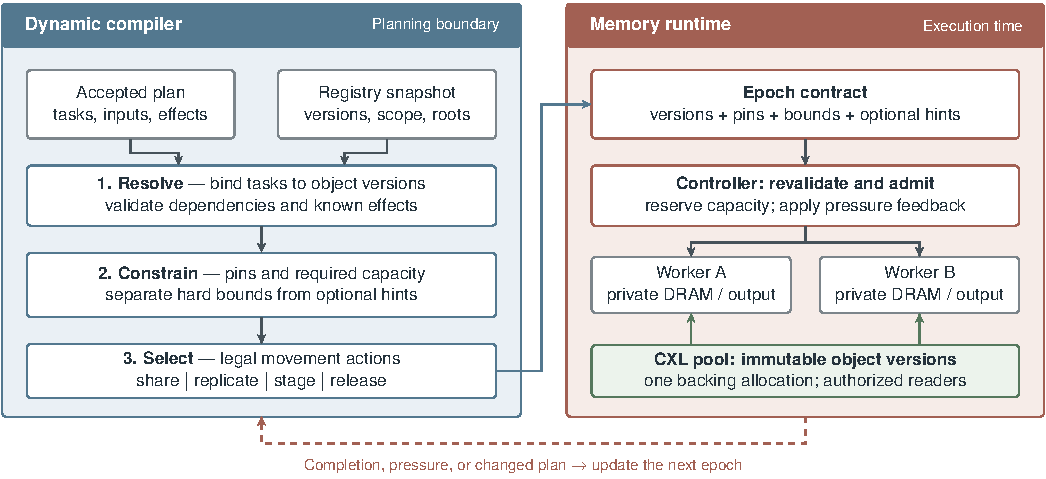
\includegraphics[width=\textwidth]{figures/architecture.pdf}
\caption{\arvm design. At a planning boundary, the compiler turns accepted
actions and registry facts into an epoch contract. The runtime revalidates
that contract, admits bounded work, and chooses placements using current
pressure. The feedback path updates later epochs. Section~\ref{sec:implementation}
distinguishes the implemented control and memory components from the full
controller design.}
\label{fig:architecture}
\end{figure*}

The memory controller checks the contract against current state, reserves
capacity, and acquires input pins before dispatch. It can reject speculative
staging while admitting an otherwise legal task. If required resources do not
fit, the task waits or takes another supported placement. This interface lets
a feedback-only policy and a plan-guided policy use the same object store.

Each component runs at a different rate. Publication, admission, and completion
update the registry. Plan boundaries and material changes trigger compilation.
Pressure sampling can throttle optional transfers between compilations.
Individual cache misses do not trigger graph updates. This keeps graph work
off the ordinary read path while retaining checks at ownership transitions.

\subsection{Design Boundary}

The design balances duplicate capacity, foreground latency, and movement cost.
A local replica may improve latency while reducing sharing density; one
session's prefetch may delay another. Contracts therefore expose required
working sets separately from optional replicas and transfers. The underlying
OS enforces mappings and isolation. \arvm relies on that substrate and targets
adapter-managed objects rather than arbitrary process memory.

\section{Data-Movement Graph and Sharing}

\subsection{Graph Representation}

For planning epoch $t$, let $G_t=(V_t,E_t)$ describe the currently resolved
operations and their dependencies. A node in $V_t$ is a task instance. A data
edge in $E_t$ references an object version produced or consumed by a task.
Control edges express ordering without implying a bulk transfer. One object
can appear on several edges without requiring several backing allocations.
Figure~\ref{fig:observed-profile} shows measured instances of these edges.
Table~\ref{tab:objects} lists the metadata needed to resolve them to backing.

\begin{table}[t]
\centering
\caption{Object information used by the compiler and runtime.}
\label{tab:objects}
\begin{tabular}{>{\raggedright\arraybackslash}p{0.27\columnwidth}>{\raggedright\arraybackslash}p{0.63\columnwidth}}
\toprule
Field & Purpose \\
\midrule
Identity and version & Recognize reuse of the same data and invalidate stale references. \\
Size and layout & Estimate capacity and transfer cost; unknown sizes are checked at runtime. \\
Producer and readers & Describe readiness, fanout, and future uses within the resolved graph. \\
Access scope & Specify which sessions or workers may map the object. \\
Mutability & Select read-only sharing, private allocation, or copy-on-write. \\
Lifetime & Track active readers, session references, and recoverable backing. \\
Placement & Record allowed memory tiers, current mappings, and device requirements. \\
\bottomrule
\end{tabular}
\end{table}

The graph uses stable object handles rather than worker-local pointers.
A handle identifies a version, an offset range, and the authority required to
resolve it. Mapping and lifetime checks remain the runtime's responsibility.
The compiler obtains these facts from retrieval adapters, tool interfaces, and
runtime object records. A free-form model plan alone is insufficient to prove
aliasing, access rights, or last use.

\subsection{What Can Be Shared}

The initial targets are immutable retrieved passages, repository snapshots,
and read-only environment data. Consumers that have permission to read the
same version can map one backing allocation. Sharing can occur across stages,
across branches, or across sessions within an authorized scope. A content hash
may help identify equal data, but equality does not grant access.

Writable objects remain private unless the runtime implements an explicit
synchronization protocol. For repository branches, a shared immutable base
with private overlays is a useful starting point. Context construction can
reuse passage references until a model backend requires a packed buffer.
That final packing or accelerator transfer is still counted as data movement.
The design makes no general assumption that model KV caches are reusable
across requests.

The runtime publishes an immutable object only after its producer completes.
It keeps active-reader references and any longer-lived session references.
A canceled branch releases its references after its running tasks stop using
them. An object absent from the current fragment may still be needed in a
later round; session retention policy or recoverable backing must cover that
case. CXL memory by itself does not provide durable storage.

\subsection{Publication, Mapping, and Reclamation}
\label{sec:protocol}

An object moves through four logical states: \emph{building},
\emph{published}, \emph{retiring}, and \emph{reclaimed}. While building, the
producer has exclusive write access and the output handle cannot be consumed.
Publication seals a version, records its length and access scope, and makes
its handle resolvable. If publication fails, the output never becomes a valid
input. Consumers acquire references only to published versions.

Retirement blocks new acquisitions while preserving existing readers. The
runtime reclaims backing only after all reader pins, mappings, device
transfers, and session roots have been discharged, or after references have
been safely redirected to an equivalent backing location. A node's completion
alone does not prove that its outputs are dead. A session root may retain a
tool transcript for a later plan even when the current DAG has no reader.
The compiler can identify a release opportunity, but the registry authorizes
the actual release.

Migration follows a prepare-and-commit protocol. The runtime first allocates
destination backing and copies a sealed version. It validates completion,
then changes the location associated with the handle for new mappings. Old
mappings remain pinned until their readers finish or acknowledge a supported
remapping operation. Only then can the old allocation be returned. During
migration both copies count against capacity. Failing to reserve this
transient double allocation can deadlock migration precisely when the pool is
under pressure.

Object generations prevent stale handles from resolving to a recycled slot.
A handle lookup validates the generation and the caller's scope before
returning a mapping. Revoking a scope blocks new mappings; existing mappings
must be drained or revoked by the OS before the allocation can be reassigned.
A software generation check cannot invalidate a pointer that a worker already
holds. The runtime therefore treats mapping teardown as a separate completion
event rather than assuming that updating the registry is sufficient.

Publication, pin management, mapping, and transient migration space all incur
costs. Sharing decisions must account for them as well as payload size.

\subsection{Placement Follows Use}

The runtime chooses among a shared CXL allocation, a local replica, and an
explicit copy to a consumer. Large objects with several readers are candidates
for shared placement. Small control records and hot private working sets may
stay in local DRAM. A local replica is useful when repeated accesses outweigh
the cost of creating and retaining it.

This choice depends on object size, access count, placement of consumers, and
measured bandwidth and latency. The compiler supplies the known dependencies;
the runtime supplies current contention and capacity. Placements use the
reported memory tiers and CPU affinity rather than fixed NUMA numbering.
Accelerator consumers use explicit staging unless their access path supports
the selected pool mapping.

\section{Dynamic Compilation of Memory Constraints}

\subsection{Compilation at Planning Boundaries}

\arvm compiles a plan when the harness has accepted a structured set of actions.
The compiler resolves known inputs, creates task instances, and links object
versions to their consumers. Unknown tool effects and input sizes retain
runtime checks. Tool completion, new retrieval results, and replanning can
trigger an update to the affected graph fragment.

The output is a memory schedule plus constraints that remain attached to it.
For example, a retrieved passage can be marked read-only and shared by two
branches; a context buffer can require local staging before a model call;
a temporary ranking buffer can be released once its last reader completes.
Compiled fragments can be reused when their shape recurs, but each reuse must
revalidate object versions, access scope, and resource bounds.

The runtime distinguishes facts from estimates. Access permissions, active
references, and backend requirements are hard constraints. Expected reuse,
branch probabilities, and predicted start times are hints. A mistaken hint
may cause an unnecessary transfer, but it must not authorize a new reader or
free an object that is still in use.

\subsection{Constraint Types}

Table~\ref{tab:constraints} summarizes the constraints and their effects on
runtime decisions.

\begin{table*}[t]
\centering
\caption{Constraints derived from a resolved plan and trusted runtime state.}
\label{tab:constraints}
\begin{tabular}{>{\raggedright\arraybackslash}p{0.16\textwidth}>{\raggedright\arraybackslash}p{0.37\textwidth}>{\raggedright\arraybackslash}p{0.39\textwidth}}
\toprule
Constraint & Meaning & Example runtime action \\
\midrule
Sharing scope & A reader must have access to the requested object version. & Map common passages read-only for authorized branches; allocate private writable outputs. \\
Lifetime & Backing must remain available while tasks or session state reference it. & Keep a tool result until synthesis completes; release it only after remaining references are resolved. \\
Placement & The object must be accessible to its admitted consumer. & Stage a model input in a supported host buffer before dispatching an accelerator transfer. \\
Capacity & Admitted work must fit within the current memory budget. & Reserve space for context packing; defer another branch if its working set does not fit. \\
Movement budget & Prefetch and migration consume limited bandwidth. & Throttle speculative staging when foreground accesses approach the configured limit. \\
Reclamation & Recall or eviction must preserve live data and active mappings. & Remove an optional local replica while retaining its backing; block reclamation of pinned buffers. \\
\bottomrule
\end{tabular}
\end{table*}

The compiler does not convert every predicted use into a permanent reservation.
It can request a short reservation for an admitted phase and a revocable hint
for a possible later phase. If an object grows beyond an estimate, the runtime
rechecks capacity before admitting its consumers. If capacity is unavailable,
it can serialize branches, delay prefetch, or choose another legal placement.
It must not reclaim live data to satisfy an optimistic plan.

\subsection{Incremental Compilation Algorithm}
\label{sec:algorithm}

The compiler keeps an index from each object version to its readers, writers,
and placements. For a plan update, it computes the affected task set and walks
only dependencies whose object identity, access mode, or admission status has
changed. Adding a reader changes the lifetime and sharing decisions for its
inputs; changing a task's private output bound changes its reservation. An
unrelated completed branch does not need to be recompiled.

Compilation has three passes. \emph{Resolve} binds logical inputs to registry
versions and checks the task's effect summary. \emph{Constrain} computes
publication dependencies, required input pins, and capacity bounds for the
admission frontier. \emph{Select} scores a small set of placements: shared
backing, a local replica, and explicit staging to the consumer. The compiler
preserves task dependencies and emits movement actions around them. It does
not rewrite the agent's reasoning or change its chosen evidence.

\begin{figure}[t]
\centering
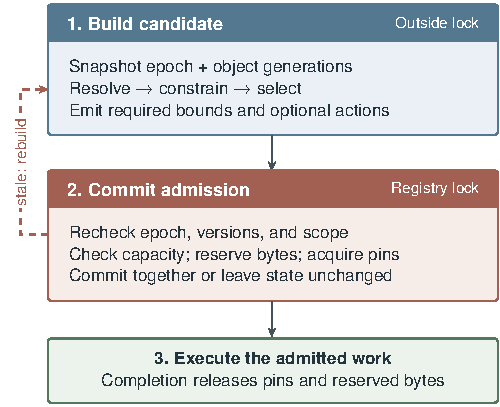
\includegraphics[width=\columnwidth]{figures/epoch.pdf}
\caption{Compile, commit, and execute. Candidate construction runs outside
the admission lock. The commit step validates the snapshot and acquires
references and capacity together; a stale candidate returns for compilation.
A rejected capacity request leaves pins and reservations unchanged.}
\label{fig:algorithm}
\end{figure}

Selection uses current measurements but does not hold the registry lock while
scoring candidates. Before admission, the runtime checks the epoch and object
generations, reserves resources, and acquires the required references as one
logical transaction. If a concurrent update changes an input, that task's
proposal is discarded. Unaffected candidates can still proceed. A small
critical section or a validated optimistic transaction can implement this
boundary; the implementation must report contention under concurrent plans.

For $v$ affected tasks, $e$ affected dependency edges, and a fixed number $k$
of candidate placements, dependency processing is $O(v+e)$ and candidate
scoring is $O(ke)$. This is a bound on the specified local algorithm, not a
claim that global scheduling is easy. Topology discovery, allocation search,
and contention can add costs. A compiler work budget bounds the time spent on each update; exceeding it
leaves the underlying feedback path in control.

\subsection{Liveness and Effect Boundaries}

A compiler can remove a buffer only when all of its possible uses within the
represented scope are accounted for. The registry distinguishes active-reader
pins, accepted-but-unstarted task references, and session roots. A branch
cancellation removes the second category after admissions stop, but it does
not remove pins held by running work. Session roots require an explicit
retention decision. Future LLM output cannot be used as a proof that old data
will never be requested again.

A retrieval adapter can often identify exact read-only inputs and a bounded
output schema. An arbitrary shell command may read or modify files that the
runtime cannot enumerate in advance. The latter receives an opaque effect
summary and keeps its private memory under the sandbox's normal accounting.
If it can modify a tracked repository region, publication of dependent
snapshots waits for the command to complete and the adapter to determine a
new version. Unknown effects reduce optimization scope rather than allowing
an optimistic alias assumption to become a correctness rule.

\subsection{Safety Properties}
\label{sec:safety}

The protocol is designed to preserve four properties. \emph{Access safety}:
a mapped version is authorized for its reader. \emph{Version stability}: a
published version's contents remain unchanged for the duration of a read.
\emph{Lifetime safety}: backing remains available while a valid mapping or
reference requires it. \emph{Capacity safety}: every admitted bounded
allocation has reserved space, including temporary migration copies.

A proof sketch follows the state transitions in
Section~\ref{sec:protocol}. Publication adds only a sealed version with a
validated scope. Acquisition checks that scope and increments a pin before
returning the mapping. Admission reserves output and staging space before
starting a consumer. Retirement prevents new acquisitions and waits for the
remaining pins and mappings. Migration retains the old backing until those
readers drain. Replanning withdraws unstarted tasks but leaves running pins
intact. Under the stated OS and adapter assumptions, each transition
preserves the four properties.

This argument specifies obligations for the implementation; it is not a
machine-checked proof of a running system. In particular, pin acquisition must
be atomic with the retirement check, and device completion must precede
release of its input buffer. Omitting either condition permits a use-after-free
execution even if graph liveness is otherwise correct. These races are
explicit targets for the validation described later.

\subsection{Constraining a MemTrade-Style Controller}

\memtrade combines a producer-side harvester with a broker that matches
available memory to consumers. Its harvester adjusts cgroup limits using
application-performance feedback; Silo buffers reclaimed pages to reduce the
cost of returning them \cite{memtrade2021}. \arvm adds an object- and
phase-level interface to this style of adaptive capacity management.

Shared identity prevents counting every graph edge as a separate allocation.
Required references constrain reassignment; predicted start times guide
optional staging. A deployment can rank legal placements by fragment time,
traffic, and local-DRAM byte-time, but admission remains authoritative and
pressure feedback remains necessary for incomplete plans.

The controller receives bounds as well as placement hints. Suppose session
$i$ has local allocation $A_i(t)$, a required resident floor $R_i(t)$ for
admitted work, and a safety margin $\Delta_i(t)$. A candidate upper bound on
capacity available for reassignment is
\begin{equation}
  H_i(t) \leq \max\{0,A_i(t)-R_i(t)-\Delta_i(t)\}.
\end{equation}
This bound is necessary but not sufficient. The allocator must identify
reclaimable allocations or replicas and preserve backing for live objects.
The runtime rejects a reduction below the floor and can tighten the bound
when observed performance deteriorates. A predicted floor is revalidated at
phase admission; it is not a proof of an opaque tool's future memory usage.

Before a phase that needs more local memory, the runtime must complete any
required recall or migration. If it cannot, the phase waits or uses a legal
alternative. Feedback remains necessary for unmodeled accesses and changes
in memory pressure. The compiler supplies lookahead; the controller decides
how much of it is worth acting on.

\memtrade is a reference for the controller design, not a CXL transport
implementation. A CXL allocator and mapping layer are required separately.
An evaluation must hold that data path constant when testing the benefit of
compiler constraints.

\subsection{Replanning and Fallback}

When a tool result changes the plan, the runtime stops admitting tasks from
the invalidated fragment and removes its unstarted speculative work. Running
tasks retain their inputs until completion or acknowledged cancellation.
The compiler updates the affected consumers, reservations, and placements,
then publishes a new epoch (Figure~\ref{fig:algorithm}). A changed object version invalidates dependent
reuse decisions.

For opaque calls, the runtime uses conservative bounds and observes actual
allocations. When compilation takes too long or has little information,
execution continues under the underlying feedback controller. Tool side
effects remain subject to harness ordering and approval. The compiler cannot
infer exactly-once external execution from a graph annotation; retries require
the tool's own idempotency or deduplication support.

\subsection{Admission, Fairness, and Pressure}
\label{sec:admission}

The controller counts physical backing once, tracks local replicas separately,
and charges every retaining session against a logical quota. Required
reservations cover admitted tasks; optional reservations may be withdrawn
before dispatch. Under pressure it cancels speculative transfers, removes
unneeded replicas after readers drain, then considers migration while
preserving live backing. If required working sets still do not fit, it reduces
admission, uses supported spilling, or reports failure.

Per-session limits bound speculation, and foreground transfers take priority.
Holding intervals and minimum predicted benefit can limit migration churn.
These are controller requirements, not measured live-adapter capabilities.
Opaque tools still require measured usage and sandbox resource limits because
a predicted memory floor cannot bound arbitrary allocations.

\subsection{Failure and Recovery}

After a worker crash, the registry releases its pins only when the OS confirms
mapping teardown and outstanding device accesses have completed or been
reset. A timeout alone is insufficient. Remaining session roots still retain
their backing. After a controller restart, reclamation must wait until
mappings and references have been reconstructed; cached plans and placement
scores can be discarded.

An unrecoverable host failure may abort the affected sessions. Recovery
across that boundary requires durable checkpoints outside the volatile CXL
pool. Restoring an object also does not authorize replaying the tool that
created it. External effects follow the harness's retry and idempotency
rules. These are recovery requirements for the full design; the component
prototype does not implement host-crash recovery.

\section{Prototype Implementation}
\label{sec:implementation}

The artifact contains an executable control-path prototype, native CXL
component benchmarks, and a live OpenCode shared-state adapter. We distinguish
the original component timings from the integrated profiling experiment;
neither implementation replaces a production sandbox memory manager.

\subsection{Control Path}

The Python registry records object generations, access scopes, session roots,
reader pins, retirement state, and reserved bytes. Admission validates the
plan epoch and input versions, checks capacity, and acquires pins under one
lock. Completion releases the reservation and pins. Reclamation requires
retirement, zero pins, and zero roots. A new publication receives a new
generation, so a recycled name does not change an existing reader's version.

The compiler validates a task DAG, resolves its distinct input handles, and
emits an admission contract. Its initial output reservation is the sum of
bounded task outputs, a conservative bound rather than optimal liveness
allocation. It supports incremental changes to output bounds when topology
and input handles are unchanged. Structural replanning takes the full
compilation path. This restriction is narrower than the general affected-
subgraph algorithm in Section~\ref{sec:algorithm}; we measure it explicitly.

The registry is trusted runtime code. It rejects unauthorized handle requests
but is not an OS isolation boundary for arbitrary Python callers. The native
data path supplies the actual read-only mapping mechanism. The live adapter
connects a separate CXL-backed registry to its own tool mappings. Extending
enforcement to opaque tools remains an integration task.

\subsection{Native Shared Objects}

The native backend creates a \texttt{memfd} object, binds its initial writable
mapping to CXL node 1, and fills it with deterministic nonzero data. It then
removes the writable mapping and seals the object against writes, growth,
and shrinkage. Workers map the published file read-only. The copy policies
instead allocate private anonymous buffers bound to DRAM node 0, copy the
same source bytes, and consume their local buffers.

The benchmark validates actual page placement from
\texttt{/proc/self/numa\_maps}; a binding request alone is not considered
successful placement. It checks the computed checksum before accepting every
observation. Process-shared barriers coordinate fanout, and independent worker
processes permit measurement of payload mappings through proportional set
size (PSS). Both policies retain the same published CXL source object.

\subsection{Phase Replay}

A second kernel executes 20 phases that consume four published object
versions in a fixed cyclic order. One reusable local slot bounds DRAM usage.
The demand policy waits through a configured planning interval, copies the
actual next input, and scans it. The lookahead policy stages a hinted input
during that interval. If the hint is wrong, it copies the actual input before
consumption. The input identity is checked independently of the hint, and
all policies must produce the same checksum.

The planning intervals and hint accuracies are controlled workload parameters,
not measured LLM behavior. This replay isolates the placement opportunity
created by lookahead. Compiler timing is measured separately and is not
included in the native phase times. Live integration must account for its
exposed cost and for contention between sessions.

\subsection{Live Shared-State Adapter}

The OpenCode adapter exposes read/search, CAS publication, and atomic append
through MCP. Its trusted tool processes map common tmpfs backing into CXL;
the model receives copied bounded text. Object metadata, grant state, pins,
and mutex words are also CXL-resident. Critical sections use the upstream
region-backed SpinLock from \texttt{mutex\_benchmark}, commit
\texttt{55b7072}; both reads and writes are exclusive. No file-lock fallback
is used. A dead lock owner causes timeout and fail-closed behavior.

Our DSec-inspired controller separates project access scopes from accepted
task effects. It pins each admitted operation and retains objects for
unstarted consumers or session roots. Task completion is reported after its
OpenCode/MCP namespace exits. Retirement blocks new pins; reclamation closes
controller mappings and unlinks backing after all relevant tasks and pins
drain. Requests outside accepted effects require a new plan. This bounded
prototype does not revoke arbitrary pointers or implement host-crash recovery.

\section{Evaluation}
\label{sec:evaluation}

We evaluate three questions: how sharing changes memory usage and data-stage
latency, when plan lookahead improves phase execution, and what the compiler
and admission checks cost. The experiments use real CXL memory and executable
kernels. The original data-stage and phase results are controlled component
benchmarks. Section~\ref{sec:live-profile} separately profiles real LLM tool
calls and two retention policies. Neither evaluates a MemTrade deployment.

\subsection{Platform and Method}

The host has an AMD Ryzen Threadripper 7960X with 24 physical cores and
48 hardware threads, running Linux 7.0.0-mk1+. A Montage CXL device
(PCI ID \texttt{1b00:c002}) reports 128\,GiB of volatile capacity. Its decoder
covers a 128\,GiB physical range; all 64 memory blocks assigned to CPU-less
NUMA node 1 fall within that range. The OS exposes approximately 15\,GiB on
node 0 and 122\,GiB on node 1 after reservations. The native code uses GCC
15.2.0 with \texttt{-O3 -march=native}; the control path uses Python 3.14.4.

Workers are pinned to distinct physical cores spread across the processor's
cache domains. Only experiment-owned source buffers are flushed before each
fanout iteration; system caches and kernel policies are unchanged. Subsequent
scans have natural cache reuse. The host is not dedicated to the experiment,
and CPU frequency is not locked. We therefore report medians and variation
rather than interpreting small differences as a stable speedup.

Node 0 has limited free memory. We bound private allocations to 32\,MiB and
check for an additional 48\,MiB free-memory margin before each configuration.
No configuration was skipped. These bounds permit controlled experiments
without creating a system-wide memory-pressure benchmark; the measurements
do not establish behavior under pool saturation or production overcommit.

\begin{table}[t]
\centering
\caption{Original component experiment coverage. Warmups are excluded;
live-agent profiling is reported separately in Section~\ref{sec:live-profile}.}
\label{tab:coverage}
\begin{tabular}{p{0.61\columnwidth}r}
\toprule
Experiment & Observations \\
\midrule
Fanout: 30 conditions, 3 policies & 2,250 \\
Phase replay: 32 conditions & 384 episodes \\
Phases per episode & 20 \\
Compiler: 5 graph sizes & 500 trials \\
Control-path test cases & 13 \\
Randomized admission/completion events & 20,000 \\
Admission/retirement race trials & 100 \\
\bottomrule
\end{tabular}
\end{table}

The fanout sweep combines 1, 4, and 8 workers; 1, 2, and 4\,MiB inputs; and
1, 4, and 16 scans, plus a single-worker 32\,MiB case at each scan count.
Each of these 30 conditions has three policies, five fresh-process blocks,
and five measured iterations per block. Every invocation also performs two
warmups. Configuration order and policy order are randomized with a recorded
seed. The phase sweep uses four blocks and three measured episodes per
configuration, also with two warmups. Raw observations, source hashes,
hardware inventory, and plotting scripts accompany the paper.

\subsection{Sharing Versus Copying}

We compare read-only CXL sharing with two copy policies. \emph{Fresh copy}
allocates and faults a new local buffer for each task. \emph{Reused copy}
retains a prefaulted local buffer across iterations, removing allocation from
the measured path. Both copy the same published CXL source before scanning.
The latter is the primary latency baseline because it avoids attributing an
allocator cost to the memory transport itself.

The timed fanout stage includes dispatch synchronization, source mapping,
required allocation and copying, and scans. It excludes process startup,
source construction, source flushing, output verification, PSS collection,
and final unmapping. We take the latest worker completion relative to the
parent's dispatch time, so scheduling delay remains included. Each checksum
and page-placement check must pass before a row enters the result set.

\begin{figure}[t]
\centering
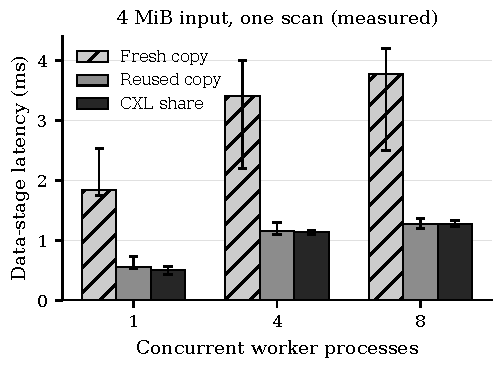
\includegraphics[width=\columnwidth]{figures/measured_fanout.pdf}
\caption{Measured data-stage latency for a common 4\,MiB input and one scan.
Bars are medians of 25 observations; whiskers span the five block medians.
Fresh allocation is costly, while sharing and reused copying are close at
eight workers. These are data-stage times, not agent response times.}
\label{fig:measured-fanout}
\end{figure}

Across the 30 conditions, the geometric mean of reused-copy median time
divided by shared median time is $1.129\times$, with a range of
$0.970$--$1.798\times$. Against fresh copying the geometric mean is
$2.606\times$. The difference between these comparisons is material:
allocation and first-touch costs account for much of the apparent advantage
against the simpler baseline.

Figure~\ref{fig:measured-fanout} shows the eight-worker 4\,MiB case at
3.778\,ms for fresh copying, 1.274\,ms for reused copying, and 1.270\,ms for
sharing. The last two distributions overlap: their interquartile ranges are
1.200--1.310\,ms and 1.218--1.296\,ms. We interpret this case as similar
latency with lower duplicate memory use. At eight workers and 16 scans of
4\,MiB, the median ratio is $0.970\times$, so sharing is slightly slower.
The data do not support a universal latency advantage.

\subsection{Memory Footprint and Placement}

For the same eight-worker input, the private payload mappings sum to
32,768\,KiB PSS. The shared source mappings, summed over workers and the
publisher, occupy approximately 4,095\,KiB PSS; integer reporting accounts
for the 1\,KiB difference from 4\,MiB. This is an eightfold difference in the
mapped payload, not in total process memory. Runtime stacks, code, registry
metadata, and other mappings are excluded from this comparison.

Both policies retain the published 4\,MiB CXL object. Thus, copying retains
that source plus 32\,MiB of private DRAM payload, while sharing retains the
source without those private copies. The private-mapping PSS number does not
include the common source again. Reporting these quantities separately avoids
using logical references as a substitute for physical memory accounting.

All accepted fanout observations report shared payload pages on node 1 and
private payload pages on node 0. All checksums match across policies. This
establishes that the experiment exercises the intended placements and data,
but it does not measure bus transactions or hardware cache-hit rates. The
benchmark uses fully overlapping inputs; partial overlap remains a workload
characterization question.

\subsection{Planning Lead Time and Wrong Hints}

The phase replay uses 8 or 32\,MiB inputs, planning intervals of 0, 0.5, 2,
and 10\,ms, and lookahead accuracies of 0\%, 50\%, and 100\%. A demand-only
policy supplies the fourth comparison at each size and interval. All policies
use a single prefaulted local slot and identical consumed object sequences.
Wrong hints are corrected before scanning, so a performance gain cannot come
from consuming less or different data.

\begin{figure}[t]
\centering
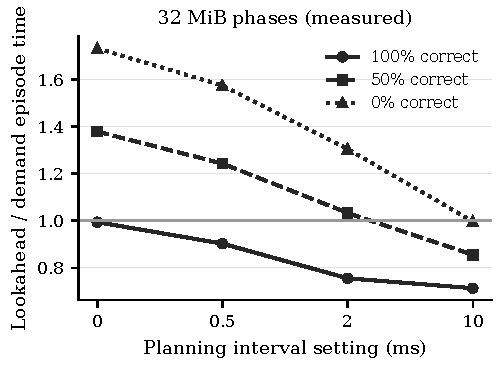
\includegraphics[width=\columnwidth]{figures/measured_phases.pdf}
\caption{Measured 20-phase episode time for 32\,MiB inputs, normalized to
demand copying at the same planning interval. Each point is a ratio of
12-observation medians. Accuracy is a controlled hint parameter; compilation
and LLM inference are not part of these timings.}
\label{fig:measured-phases}
\end{figure}

With 32\,MiB inputs and a 2\,ms planning interval, correct lookahead reduces
median episode time from 159.428\,ms to 120.515\,ms, a 24.4\% reduction.
At a 10\,ms interval, times are 312.905\,ms and 223.381\,ms, a 28.6\%
reduction. These reductions come from moving copies into the available
interval; the benchmark does not shorten the configured interval itself.

Wrong hints expose the cost of treating every prediction as a reservation.
With no lead time and 0\% accuracy, median time rises from 119.049\,ms to
206.036\,ms for 32\,MiB inputs, a 73.1\% increase. The copy volume doubles
from 640\,MiB to 1,280\,MiB per episode. At 50\% accuracy, copy volume is
960\,MiB. With a 10\,ms interval, wrong prefetch can fit inside the available
wait and leave latency near the demand baseline, but the doubled traffic
remains. A controller that measures latency alone would miss that cost.

The source pool is flushed before each episode, not before each phase.
Later phases therefore retain natural cache reuse. The two object sizes
produce different working sets; Figure~\ref{fig:measured-phases} measures
the scheduling mechanism under these conditions, not pure link bandwidth.

\subsection{Compiler and Admission Overhead}

The control benchmark uses four-way task trees with 16, 64, 256, 1,024, and
4,096 nodes. Every graph references one common immutable input and gives each
task a bounded output. Each size has 100 trials. We separately time full
compilation, changing one leaf's output bound, and admitting the resulting
contract. Task construction and native execution are outside these timers.

\begin{figure}[t]
\centering
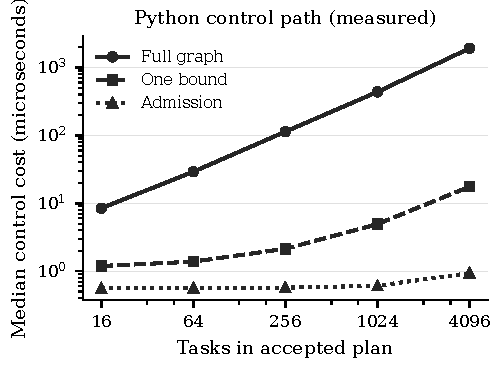
\includegraphics[width=\columnwidth]{figures/measured_compiler.pdf}
\caption{Measured Python control costs, with 100 trials per graph size.
Both axes use logarithmic scales. The incremental operation changes one
output bound without changing topology; admission pins one distinct input.}
\label{fig:measured-compiler}
\end{figure}

Full compilation takes a median 8.448\,$\mu$s at 16 nodes,
113.347\,$\mu$s at 256 nodes, and 1.908\,ms at 4,096 nodes. A single-bound
update takes 1.191, 2.133, and 17.532\,$\mu$s at those sizes. Admission
medians range from 0.561 to 0.936\,$\mu$s. The admission result reflects one
distinct input handle; it is not a bound for many-object admission or registry
contention.

These costs support a bounded compilation strategy. Small accepted fragments
can be inexpensive relative to millisecond transfers, but compiling thousands
of tasks can consume much of a short planning interval. Structural changes
still take the full path in this prototype. A live implementation should
measure the exposed cost after overlap and use fallback when the compilation
budget is exceeded, rather than assuming every replan is cheap.

\subsection{Live Agent Sharing and Dataflow Ablation}
\label{sec:live-profile}

We run OpenCode v2.0.24 against local Qwen3.5-35B-A3B, quantized as
UD-Q4\_K\_XL, on an RTX 5090. Two 16K-context model slots serve two or four
reviewer roles. Each role runs a fresh task session in each of two rounds;
a final session synthesizes their results. The common input is a
\ProfileCorpusKiB\,KiB snapshot of four actual prototype modules.
The harness specifies accepted effects and broad project read scopes.
The model executes source searches, publications, peer reads,
and ledger appends. This measures execution of a known fragment, not natural
plan discovery or independent answer quality.

Two policies use identical allocation bounds, permissions, and CXL locks.
\emph{Scope-only} retains any object that a pending task is authorized to
read. \emph{Dataflow} retains objects named by accepted future effects,
current pins, or session roots. Both reject operations outside the accepted
effects; introducing such a use requires replanning. Each worker-count/policy
pair has three trials in randomized blocks: \ProfileEpisodes{} episodes,
\ProfileSessions{} task sessions, and \ProfileEvents{} recorded operations.
All episodes publish their outputs; \ProfileProtocol{} follow every required
tool step. One scope-only synthesis omits the requested pre-write read of
\texttt{answer}; its CAS publication succeeds. Every attempt is retained.

\textbf{Physical sharing.} All readers resolve the source to the same device
and inode, with every resident payload and mutex page verified on CXL node 1.
A separate three-repeat concurrent mapping probe holds every mapping alive
while sampling PSS. Shared source mappings sum to 64\,KiB with either two or
four workers. Retaining the same source plus per-worker DRAM copies uses
192 and 320\,KiB, respectively. This is a payload-mapping measurement; model,
interpreter, registry, and RPC buffers are outside that PSS sum.

\textbf{Retention.} Payloads use fixed 64\,KiB slots, including unused bounded
output capacity. We integrate allocated payload bytes over the observed task
interval and divide by that interval to obtain average occupancy. Dataflow
actually unlinks dead backing after task namespaces and pins drain; source,
draft, and review objects remain until their accepted readers finish.
Table~\ref{tab:live-retention} reports trial medians. Replaying scope-only
retention on each dataflow trial's own timestamps yields median byte-time
reductions of \ProfileTwoReplaySaving\% and \ProfileFourReplaySaving\%,
separating lifetime decisions from differences in model execution time.
That replay is a capacity calculation, not another latency measurement.

\begin{table}[t]
\centering
\caption{Measured average live CXL payload. Three trials per cell;
64\,KiB slots include unused reserved output space. Registry/lock storage
is accounted separately in the artifact.}
\label{tab:live-retention}
\begin{tabular}{rrrr}
\toprule
Reviewers & Scope-only & Dataflow & Reduction \\
 & KiB & KiB & \\
\midrule
2 & \ProfileTwoScopeKiB & \ProfileTwoGraphKiB & \ProfileTwoSaving\% \\
4 & \ProfileFourScopeKiB & \ProfileFourGraphKiB & \ProfileFourSaving\% \\
\bottomrule
\end{tabular}
\end{table}

\begin{figure*}[t]
\centering
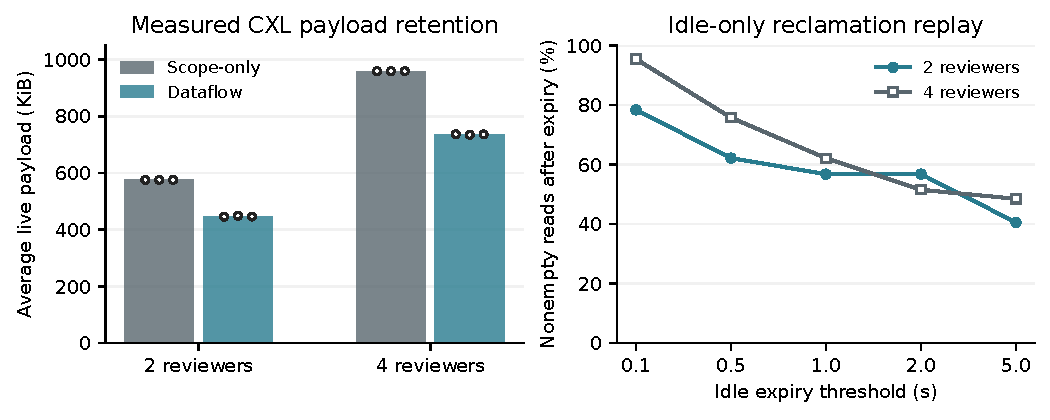
\includegraphics[width=\textwidth]{figures/profile-sharing-profile.pdf}
\caption{Left: measured retention, with median bars and every trial shown.
Right: hypothetical idle-only reclamation replayed on all six dataflow
episodes. A read is at risk when its preceding inter-access gap exceeds the
threshold. No unsafe eviction is executed, and no observed crash is claimed.}
\label{fig:live-retention}
\end{figure*}

\textbf{Why activity alone is insufficient.} With a one-second idle threshold,
\ProfileIdleOneReads{} of \ProfileIdleOneDenominator{} nonempty reads
(\ProfileIdleOnePercent\%) follow an expired interval. This replay counts
future accesses requiring retained or recoverable backing, not actual
use-after-free failures. Scope-only retention is safe but conservative;
idle-only reclamation lacks a future-use guarantee. Object-version dataflow
provides the missing distinction. Equivalent reference tables may provide it
as well. Small prescribed tasks, fixed slot sizes, and two model slots limit
generality. We report no causal inference-speedup or total-process-memory claim.


\subsection{Correctness Checks and Limits}

All 13 control-path tests pass. They cover unauthorized readers, unknown
generations, name reuse, retirement with live readers, capacity rejection
without partial pinning, duplicate references, stale epochs, cyclic graphs,
missing dependencies, incremental bounds, and repeated completion. The suite
also runs 100 admission/retirement races and 20,000 randomized admission and
completion events, checking reservation bounds and reference conservation.
These tests exercise the executable registry; they do not constitute a proof
of OS isolation or crash recovery.

The native experiments contribute 2,250 fanout observations and 384 phase
episodes with matching checksums and verified placement. The original
compiler and native memory timings remain component measurements.
The live adapter adds real-model execution of prescribed fragments and 12
additional tests, including CXL lock failure, effect/scope separation,
future-use retention, and physical reclamation. Natural plan discovery,
opaque-tool coverage, many-session contention, recall of leased capacity,
and a tuned feedback-controller comparison remain open. The demand-copy
baseline is not a reproduction of MemTrade; NVIDIA Sentry has not been
measured on this host.

The measured result is a capacity benefit with workload-dependent data-stage
latency, plus a lookahead opportunity that can disappear or reverse under
wrong or late hints. The sample counts support these component comparisons;
they do not support production p99 latency or availability claims.

\section{Related Work}
\label{sec:related}

\textbf{Agents and RAG.} RAG connects retrieval to generation
\cite{rag2020}, and ReAct interleaves reasoning with external actions
\cite{react2023}. MUSE and DSec supply the workload motivation discussed in
Section~2. Our graph describes the data retained between these operations.
The proposal does not change retrieval quality, model reasoning, or tool
selection; those remain fixed when measuring movement-policy effects.

\textbf{Workflow communication and compilation.} SONIC selects data passing
and placement for serverless workflow edges \cite{sonic2021}. Faastlane
reduces interaction cost through shared-process execution when suitable,
with isolation and other execution modes when needed \cite{faastlane2021}.
SkVM compiles skills for model and harness capabilities and extracts workflow
concurrency \cite{skvm2026}. \arvm instead takes accepted task fragments as
input and derives object-sharing and memory-admission contracts. The relevant
boundary is between task dependencies and physical memory lifetime, including
references that survive a replan.

\textbf{Shared disaggregated memory.} Duhu provides an object store for data
processing frameworks over shared disaggregated memory and integrates it with
Ray \cite{duhu2026}. MEGALON supports sharing when only part of a CXL region
is coherent \cite{megalon2026}. These mechanisms address the memory substrate.
\arvm addresses which versions an accepted plan needs, which uses permit
sharing, and when placement changes are legal. Evaluating the plan interface
above the same substrate is necessary to isolate its contribution.

\textbf{Memory harvesting and tiering.} \memtrade studies harvesting and
matching idle memory in public clouds \cite{memtrade2021}. TPP studies
transparent placement for CXL tiered memory, while AIFM and Semeru expose
remote memory through application and managed-runtime interfaces
\cite{tpp2023,aifm2020,semeru2020}. \arvm proposes supplying agent dependencies
and lifetimes to resource-management decisions. It retains runtime feedback
for unobserved accesses and pressure changes. The appropriate comparison uses
the same capacity and memory data path, avoiding a claim that a CXL transport
advantage demonstrates a better controller.

\section{Conclusion}\label{sec:conclusion}

\arvm makes the memory requirements of accepted agent plans explicit:
which versions can be shared, which references must remain live, and which
inputs can be staged before use. Compilation supplies this information;
admission validates it against current state and capacity. Native CXL
measurements show that sharing can remove private copies at similar latency,
while lookahead trades exposed transfer time against the cost of wrong hints.
Live multi-round agent traces additionally show why permissions and activity
alone are insufficient for precise shared-state retention: accepted object
uses permit earlier release while preserving later consumers. The results
support these mechanisms. Natural workloads and a comparison with tuned
feedback-based capacity management are still needed to establish the full
system benefit.

\clearpage
\label{page:references}
\bibliographystyle{plain}
\bibliography{references}

\end{document}
